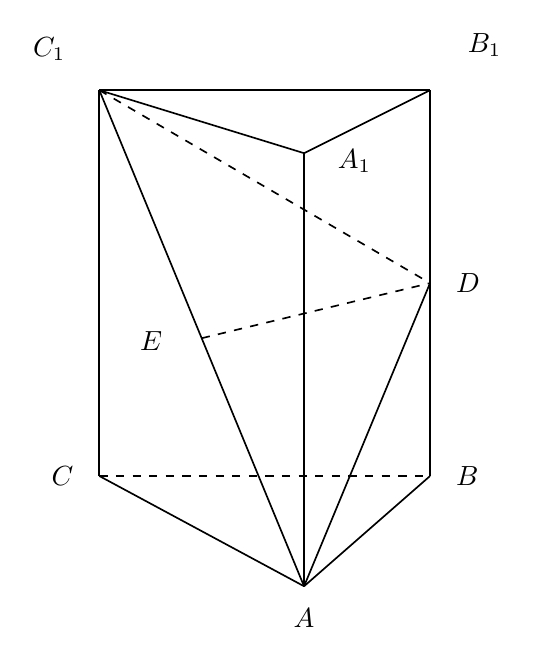
\begin{tikzpicture}[x=1cm,y=1cm,line width=.6pt,font=\normalsize,
  geometry edge/.style={solid,line width=.6pt},
  geometry label/.style={font=\normalsize,inner sep=2pt}]
% Straight triangular prism ABC-A1B1C1, oblique schematic projection.
% D is midpoint of BB1, E is midpoint of AC1.
\coordinate (C1) at (0,5.5);
\coordinate (B1) at (4.2,5.5);
\coordinate (A1) at (2.6,4.7);
\coordinate (A) at (2.6,-0.8);
\coordinate (C) at (0,0.6);
\coordinate (B) at (4.2,0.6);
\coordinate (D) at (4.2,3.05);
\coordinate (E) at (1.3,2.35);
% Visible solid edges
\draw[geometry edge] (C1)--(B1);
\draw[geometry edge] (B1)--(A1);
\draw[geometry edge] (B1)--(B);
\draw[geometry edge] (C1)--(C);
\draw[geometry edge] (C1)--(A);
\draw[geometry edge] (A1)--(A);
\draw[geometry edge] (A)--(D);
\draw[geometry edge] (A)--(C);
\draw[geometry edge] (A)--(B);
% Hidden edges (dashed)
\draw[geometry edge,dashed] (C)--(B);
\draw[geometry edge] (C1)--(A1);
\draw[geometry edge,dashed] (C1)--(D);
\draw[geometry edge,dashed] (E)--(D);
% Labels placed clear of all strokes
\node[geometry label,anchor=south east] at (-0.35,5.8) {$C_{1}$};
\node[geometry label,anchor=south west] at (4.6,5.85) {$B_{1}$};
\node[geometry label,anchor=west] at (2.95,4.6) {$A_{1}$};
\node[geometry label,anchor=east] at (0.88,2.32) {$E$};
\node[geometry label,anchor=west] at (4.45,3.05) {$D$};
\node[geometry label,anchor=east] at (-0.25,0.6) {$C$};
\node[geometry label,anchor=west] at (4.45,0.6) {$B$};
\node[geometry label,anchor=north] at (2.6,-1.0) {$A$};
\end{tikzpicture}
